
%\documentclass[manuscript]{acmart}
%\documentclass[acmsmall]{acmart}
%\settopmatter{printacmref=false}


\documentclass[
  a4paper,
  12pt,
  DIV=12,        % höherer Wert = schmalere Ränder, weniger Whitespacmi
  parskip=half,  % Absätze mit halbem Abstand statt Einzug
  headings=small % kleinere Überschriften, weniger vertikaler Abstand
]{scrartcl}

%\documentclass[a4paper,11pt]{scrartcl}
%\documentclass[a4paper,11pt]{report}
%\documentclass[a4paper,12pt]{book}
\usepackage[utf8]{inputenc}
\usepackage[german]{babel}
\usepackage[T1]{fontenc}
\usepackage{lmodern}
\usepackage[inkscapelatex=false]{svg}
% Texte im SVG von Inkscape setzen lassen, nicht durch die Dokumentschrift ersetzen
\svgsetup{inkscapelatex=false}
\usepackage{amsmath}
\usepackage{caption}
\usepackage{gensymb}
\usepackage{microtype}
\usepackage{longtable}
\usepackage{tabularx}   % Spalten, die die restliche Zeilenbreite auffüllen (X-Spalte)
\usepackage{booktabs}   % \toprule \midrule \bottomrule (in mobrob_table.tex verwendet)
\usepackage{wrapfig}    % Textumfluss um Abbildungen
\usepackage{array}
\usepackage{calc}

\usepackage[citecolor=black, colorlinks=true, linkcolor=black, urlcolor=blue]{hyperref}


%\usepackage{geometry}
\usepackage{siunitx}
%\geometry{margin=2.5cm}


\usepackage{amsthm}
\usepackage{mdframed}
\usepackage{enumitem}

\newmdtheoremenv{theorem}{Theorem}

\theoremstyle{definition}
\newmdtheoremenv{derivation}{Derivation}

\providecommand{\tightlist}{%
  \setlength{\itemsep}{0pt}\setlength{\parskip}{0pt}}

%\mdfdefinestyle{leftline}{
%    topline=false, bottomline=false, rightline=false,
%    linewidth=2pt, linecolor=gray
%}
\theoremstyle{definition}
\newmdtheoremenv[style=leftline]{myalgorithm}{Algorithm}




%\usepackage{fancyvrb}







\let\Bbbk\relax
\usepackage{amssymb}


\usepackage{yfonts}

\usepackage{kvmap}

\usepackage[
    backend=biber,
    style=alphabetic,
    sortlocale=de_DE,
    natbib=true,
    %url=false,
    doi=true,
    %eprint=false
]{biblatex}
% \addbibresource{Literaturrecherche-Stefan-Etringer/algo-references.bib}

%\usepackage[
%    backend=biber,
%    style=alphabetic,
%    sortlocale=de_DE,
%    natbib=true,
%    %url=false,
%    doi=true,
%    %eprint=false
%]{biblatex}
%\addbibresource{Literaturrecherche-Dennis/mobrob_references.bib}

\usepackage[autostyle=true,german=quotes]{csquotes}
\usepackage{trfsigns} %fourier transform arrow
\usepackage{mathrsfs} %fourier F
\usepackage{commath}

\usepackage{pgfplots}
\pgfplotsset{compat=1.18}

\usepackage{xcolor}
\usepackage{listings}
\usepackage[european]{circuitikz}
\ctikzset{tripoles/european not symbol=ieee circle}

%\usepackage[shading]{moeptikz}
%\moeptikzset{shading=true}

%\usepackage{german,longtable}

\usepackage{xcolor}
\usepackage{color}
\usepackage{url}

\usepackage{xfrac}

\usepackage{listings}
\usepackage{verbatimbox}

\usepackage{algorithm}
\usepackage{algpseudocode}

\usepackage{multirow}
\usepackage{float}
\usepackage{pdflscape}   % einzelne Querformatseiten (im PDF gedreht)

%%%% TIKZ

\usepackage{tikz}

\usepackage{pgfplots}
\usetikzlibrary{calc,
trees,positioning,arrows,
chains,shapes.geometric,
decorations.pathreplacing,
decorations.pathmorphing,shapes,
matrix,shapes.symbols,
plotmarks}
%\tikzexternalize[prefix=figures/]

%\tikzset{%
%  block/.style    = {draw, thick, rectangle, minimum height = 3em,
%    minimum width = 3em},
%  sum/.style      = {draw, circle, node distance = 2cm}, % Adder
%  input/.style    = {coordinate}, % Input
%  output/.style   = {coordinate} % Output
%}
% Defining string as labels of certain blocks.
%\newcommand{\suma}{\Large$+$}
%\newcommand{\multa}{\Large$\times$}
%\newcommand{\inte}{$\displaystyle \int$}
%\newcommand{\derv}{\huge$\frac{d}{dt}$}

\usetikzlibrary{arrows,automata,positioning}
%\usepackage{automata}


%%% END TIKZ

\usepackage[section]{placeins}

\usepackage{textcomp}


\usepackage{listings}
\usepackage{verbatimbox}

\usepackage{bold-extra}

\usepackage{framed}

%\usepackage{fancyhdr}
%\pagestyle{fancy}
%\lhead{\leftmark}
%\chead{}
%\rhead{}
%\lfoot{}
%\cfoot{\thepage}
%\rfoot{}
%\renewcommand{\headrulewidth}{0.2pt}
%\renewcommand{\footrulewidth}{0.2pt}



\newcommand{\Z}{\mathbb{Z}}
\newcommand{\R}{\mathbb{R}}
\newcommand{\C}{\mathbb{C}}
\newcommand{\N}{\mathbb{N}}
\newcommand{\SqrtNy}{$\sqrt{\textsc{Ny}}$}
\newcommand{\conj}{\overline}
\newcommand{\Kset}{\textswab{K}}
\newcommand{\Qset}{\textswab{Q}}
\newcommand{\ceil}[1]{\left\lceil #1 \right\rceil}
\newcommand{\floor}[1]{\left\lfloor #1 \right\rfloor}
\newcommand{\sorted}[1]{\textsc{sort}\left\lbrace #1 \right\rbrace}
\newcommand{\SNRgain}{a_{SNR}}
\newcommand{\EQgain}{a_{EQ}}
\newcommand{\SIRgain}{a_{SIR}}
\newcommand{\SNIRgain}{a_{SINR}}
\newcommand{\SNR}{\textsc{SNR}}
\newcommand{\CIRgain}{a_{CIR}}
\newcommand{\CINRgain}{a_{CINR}}
\newcommand{\CNR}{\textsc{CNR}}
\newcommand{\CINR}{\textsc{CINR}}
\newcommand{\HPAModel}{ Hughes 1177H TWTA }
\newcommand{\bigO}{\mathcal{O}}
\newcommand{\CopWinCompl}{2.375377}
\newcommand{\IBO}{\textsc{IBO}}
\newcommand{\OBO}{\textsc{OBO}}
\newcommand{\spacepage}{\newpage\null\thispagestyle{empty}\newpage}
\newcommand{\satcom}{ SatCom }
\newcommand{\db}{~\text{dB}}


\definecolor{mGreen}{rgb}{0,0.6,0}
\definecolor{mGray}{rgb}{0.5,0.5,0.5}
\definecolor{mPurple}{rgb}{0.58,0,0.82}
\definecolor{backgroundColour}{rgb}{0.95,0.95,0.92}

\lstdefinestyle{CStyle}{
    backgroundcolor=\color{backgroundColour},
    commentstyle=\color{mGreen},
    keywordstyle=\color{magenta},
    numberstyle=\tiny\color{mGray},
    stringstyle=\color{mPurple},
    basicstyle=\footnotesize,
    breakatwhitespace=false,
    breaklines=true,
    captionpos=b,
    keepspaces=true,
    numbers=left,
    numbersep=5pt,
    showspaces=false,
    showstringspaces=false,
    showtabs=false,
    tabsize=2,
    language=C
}

\lstdefinelanguage{VHDL}{
  morekeywords=[1]{library,use,all,entity,is,port,in,out,end,architecture,of,begin,process,if,then,else,elsif,when,others,signal,variable,wait,for,loop},
  morecomment=[l]--,
  morestring=[b]",
  sensitive=true
}

\lstset{
  language=VHDL,
  basicstyle=\ttfamily\small,
  keywordstyle=\color{blue},
  commentstyle=\color{gray},
  stringstyle=\color{red},
  numbers=left,
  numberstyle=\tiny,
  stepnumber=1,
  numbersep=8pt,
  frame=single,
  breaklines=true,
  captionpos=b
}

\lstset{numbers=none}

%\newcounter{example}
%\renewcommand{\theexample}{\thesection.\arabic{example}}


% Default fixed font does not support bold face
\DeclareFixedFont{\ttb}{T1}{txtt}{bx}{n}{12} % for bold
\DeclareFixedFont{\ttm}{T1}{txtt}{m}{n}{12}  % for normal

% Custom colors
\usepackage{color}
\definecolor{deepblue}{rgb}{0,0,0.5}
\definecolor{deepred}{rgb}{0.6,0,0}
\definecolor{deepgreen}{rgb}{0,0.5,0}

\usepackage{listings}

% Python style for highlighting
\newcommand\pythonstyle{\lstset{
language=Python,
basicstyle=\ttm,
morekeywords={self},              % Add keywords here
keywordstyle=\ttb\color{deepblue},
emph={MyClass,__init__},          % Custom highlighting
emphstyle=\ttb\color{deepred},    % Custom highlighting style
stringstyle=\color{deepgreen},
frame=tb,                         % Any extra options here
showstringspaces=false
}}


% Python environment
\lstnewenvironment{python}[1][]
{
\pythonstyle
\lstset{#1}
}
{}

% Python for external files
\newcommand\pythonexternal[2][]{{
\pythonstyle
\lstinputlisting[#1]{#2}}}

% Python for inline
\newcommand\pythoninline[1]{{\pythonstyle\lstinline!#1!}}





\nocite{*}


\begin{document}
%\pagenumbering{roman}



\title{Coasterbot}
\subtitle{Lastenheft}
\author{Stefan Etringer}
%\email{gereonsuch@suchdsp.com}
%\affiliation{
%  \institution{Wilhelm Büchner University of Applied Sciences}
%  \department{Computer Engineering}
%  \city{Hof}
%  \country{Germany}
%}



\begin{titlepage}
  \begin{center}
    {\large Wilhelm Büchner University of Applied Sciences} \\[0.3em]

    {\normalsize Projektseminar Master}
\vspace{5em}

    {\LARGE\bfseries Coasterbot} \\[0.5em]

    {\large Phasenpaper M0} \\[1em]

    {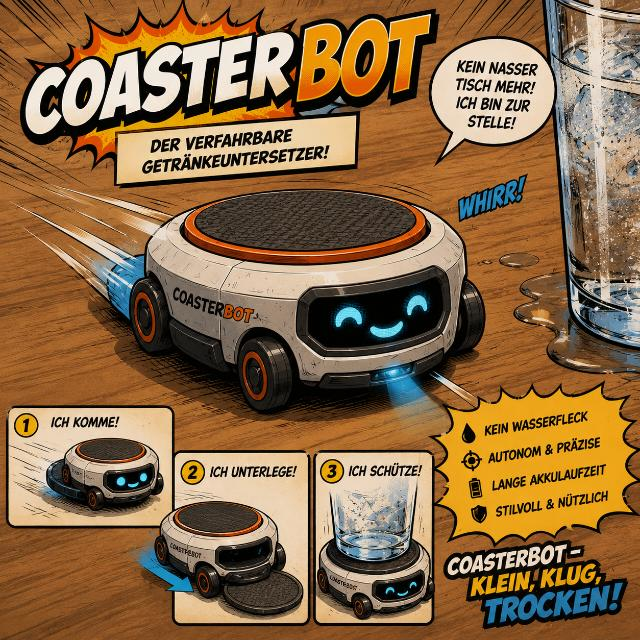
\includegraphics[width=0.38\textwidth]{coasterbot.png}} \\[1em]

\vspace{4em}

    {\normalsize
\begin{tabular}{ll}
Dennis Borutta, B. Eng & dennis.borutta@outlook.com\\
Stefan Etringer, B. Eng & mail@stefan.works\\
Gereon Such, M. Sc. & gereonsuch@gmail.com\\
\end{tabular}
    }
  \end{center}


\end{titlepage}


% einleitung preambel etc.


% Versionshistorie des Dokuments -- eigene Seite direkt nach dem Titelblatt
\section*{Versionshistorie}

\begin{tabularx}{\textwidth}{@{}clp{2.6cm}X@{}}
\toprule
\textbf{Version} & \textbf{Datum} & \textbf{Bearbeiter} & \textbf{Änderungen}\\
\midrule
1 & 05.08.2026 & Etringer & Erstfassung des Lastenhefts\\
\bottomrule
\end{tabularx}


\newpage

\tableofcontents

\newpage

\section{1 Einleitung}\label{einleitung}

\subsection{1.1 Ausgangssituation}\label{ausgangssituation}

Die Gastronomie steht seit mehreren Jahren vor erheblichen personellen
Herausforderungen. Insbesondere der anhaltende Fachkräftemangel
erschwert den wirtschaftlichen Betrieb vieler Restaurants, Bars und
Cafés. Mitarbeitende müssen neben der eigentlichen Betreuung der Gäste
zahlreiche wiederkehrende Tätigkeiten übernehmen, beispielsweise das
Verteilen und Einsammeln von Getränkeuntersetzern. Obwohl diese Aufgaben
keinen hohen fachlichen Anspruch besitzen, binden sie Arbeitszeit und
reduzieren die verfügbare Zeit für den direkten Gästeservice.

Parallel dazu gewinnen autonome mobile Robotersysteme zunehmend an
Bedeutung. Fortschritte in den Bereichen Sensorik, eingebettete Systeme
und Machine Learning ermöglichen den Einsatz kleiner autonomer Roboter
auch in dynamischen Umgebungen. Während bereits Serviceroboter für den
Transport von Speisen oder Getränken existieren, existieren bislang nur
wenige spezialisierte Systeme für kleinere Serviceaufgaben auf dem
Tisch.

Vor diesem Hintergrund soll ein kompakter autonomer Roboter entwickelt
werden, der Getränkeuntersetzer selbstständig zu Gästen bringt, unter
Getränken platziert und nach Gebrauch wieder aufnimmt. Der entwickelte
Prototyp dient als Machbarkeitsnachweis für dieses Konzept.

\subsection{1.2 Projektziel}\label{projektziel}

Ziel dieses Projekts ist die Entwicklung eines Prototyp, nämlich des
\emph{Coasterbots}. Dabei handelt es sich um einen ca. handtellergroßen
autonomen mobilen Roboter, der sich auf einer Tischoberfläche
selbstständig bewegt und Getränkeuntersetzer automatisiert verteilt
sowie wieder einsammelt.

Im Rahmen der Projektarbeit liegt der Schwerpunkt auf der Entwicklung
einer geeigneten Systemarchitektur sowie der Konzeption der
erforderlichen Softwarekomponenten. Zusätzlich werden die mechanischen
und elektronischen Komponenten des Prototyps so ausgearbeitet, dass eine
Fertigung grundsätzlich möglich ist. Zur Absicherung des Systementwurfs
wird eine Simulation entwickelt, mit der die wesentlichen Funktionen des
Roboters reproduzierbar getestet und validiert werden können.

Der Fokus der Arbeit liegt nicht auf der Entwicklung eines serienreifen
Produkts, sondern auf dem Nachweis der technischen Realisierbarkeit der
Kernfunktionen.

\subsection{1.3 Projektumfang}\label{projektumfang}

Der Projektumfang umfasst die Entwicklung eines Prototyps mit den für
den Funktionsnachweis erforderlichen Eigenschaften. Hierzu gehören
insbesondere:

\begin{itemize}
\tightlist
\item
  Konzeption der Sensorik und Aktorik.
\item
  Erstellung der mechanischen Konstruktion einschließlich der
  erforderlichen STL-Dateien.
\item
  Konzeption der Navigations- und Lokalisierungsfunktionen.
\item
  Entwicklung einer modularen Softwarearchitektur.
\item
  Entwicklung der Softwarekomponenten zur Steuerung des Roboters.
\item
  Erstellung der elektronischen Schaltpläne.
\item
  Entwicklung einer Simulationsumgebung zur Validierung der Software.
\item
  Identifikation und Definition der aus den Anforderungen resultierenden
  Testfälle.
\end{itemize}

Die funktionalen Anforderungen konzentrieren sich auf die Kernfunktionen
der autonomen Navigation, der Handhabung von Getränkeuntersetzern, der
Systemsicherheit sowie der Systemüberwachung. Erweiterte Funktionen
werden als zukünftige Ausbaustufen betrachtet.

\subsection{1.4 Projektabgrenzung}\label{projektabgrenzung}

Nicht Bestandteil dieses Projekts sind Funktionen, die über den Nachweis
der grundlegenden technischen Machbarkeit hinausgehen. Insbesondere sind
folgende Themen nicht Gegenstand der Projektarbeit:

\begin{itemize}
\tightlist
\item
  Betrachtungen zur elektromagnetischen Verträglichkeit (EMV).
\item
  Kartierung oder dauerhafte Modellierung der Umgebung.
\item
  Einbindung des Systems in Netzwerke oder Cloud-Dienste.
\item
  Marketing- und Wirtschaftlichkeitskonzepte.
\item
  Koordination mehrerer Coasterbots (Schwarmverhalten).
\item
  Vollständige Automatisierung von Bestell- oder Bezahlvorgängen.
\item
  Automatisierte Tischreinigung.
\item
  Getränketransport als Primärfunktion des Systems.
\end{itemize}

Die genannten Funktionen stellen mögliche Erweiterungen zukünftiger
Entwicklungsstufen dar und werden im Rahmen dieser Projektarbeit nicht
umgesetzt.

\subsection{1.5 Zielgruppe des
Lastenhefts}\label{zielgruppe-des-lastenhefts}

Dieses Lastenheft beschreibt die Anforderungen an den zu entwickelnden
Coasterbot aus Sicht des Auftraggebers. Es dient als Grundlage für die
Systementwicklung sowie für die Erstellung des Pflichtenhefts, der
Systemarchitektur, der Simulation und der späteren Testfälle. Darüber
hinaus bildet es die Basis für die Nachverfolgbarkeit der Anforderungen
während des gesamten Entwicklungsprozesses.

\section{2 Systemübersicht}\label{systemuxfcbersicht}

\subsection{2.1 Systembeschreibung}\label{systembeschreibung}

Der Coasterbot ist ein autonomes, mobiles Robotersystem, das auf
Tischoberflächen eingesetzt wird. Seine Hauptaufgabe besteht darin,
Getränkeuntersetzer selbstständig zu Gästen zu transportieren, diese
präzise unter Getränken zu platzieren und nach Gebrauch wieder
aufzunehmen. Der Bot bewegt sich dabei eigenständig innerhalb des ihm
zur Verfügung stehenden Arbeitsbereichs und erkennt Hindernisse sowie
die Begrenzungen der Tischoberfläche.

Der Coasterbot ist als kompakter Prototyp konzipiert und dient dem
Nachweis der technischen Machbarkeit des beschriebenen Anwendungsfalls.
Die Entwicklung umfasst sowohl die mechanische Konstruktion als auch die
Elektronik sowie die Softwarearchitektur einschließlich einer
Simulationsumgebung zur Validierung des Systemverhaltens.

\subsection{2.2 Systemkontext}\label{systemkontext}

Der Coasterbot wird in gastronomischen Einrichtungen wie Restaurants,
Cafés oder Bars eingesetzt. Während des Betriebs befindet sich der
Roboter ausschließlich auf einer Tischoberfläche und interagiert mit
Gästen sowie mit den auf dem Tisch befindlichen Objekten.

Die Systemgrenze umfasst sämtliche Hard- und Softwarekomponenten des
Roboters. Nicht Bestandteil des Systems sind externe Informationssysteme
wie Kassensysteme, Warenwirtschaftssysteme oder Cloud-Dienste. Ebenso
gehören Personen und die physische Umgebung nicht zum System, sondern
stellen externe Akteure beziehungsweise Randbedingungen dar.

Die Interaktion des Systems erfolgt mit folgenden externen Entitäten:

\begin{itemize}
\tightlist
\item
  Gäste, die Getränkeuntersetzer anfordern oder entgegennehmen.
\item
  Servicepersonal, das den Bot startet, überwacht oder wartet.
\item
  Getränke und Getränkeuntersetzer als zu handhabende Objekte.
\item
  Tischoberfläche als Arbeitsbereich des Roboters.
\item
  Hindernisse wie Gläser, Teller oder Dekorationselemente.
\end{itemize}

\subsection{2.3 Einsatzbereich}\label{einsatzbereich}

Der Coasterbot ist ausschließlich für den Betrieb auf ebenen
Tischoberflächen in Innenräumen vorgesehen. Der Einsatz erfolgt in einer
kontrollierten Umgebung mit ausreichend Beleuchtung und einer für
gastronomische Einrichtungen üblichen Anordnung von Getränken und
Gegenständen.

Der Roboter ist nicht für den Einsatz auf unebenen Flächen, im
Außenbereich oder unter extremen Umgebungsbedingungen vorgesehen. Ebenso
ist kein Betrieb auf mehreren Tischen oder ein Wechsel zwischen
unterschiedlichen Tischen vorgesehen.

\subsection{2.4 Anwender}\label{anwender}

Das System besitzt unterschiedliche Nutzergruppen mit verschiedenen
Aufgaben.

\subsubsection{Gäste}\label{guxe4ste}

Gäste interagieren indirekt mit dem Coasterbot, indem sie
Getränkeuntersetzer anfordern oder entgegennehmen. Darüber hinaus
erhalten sie Statusinformationen über den aktuellen Arbeitszustand des
Roboters.

\subsubsection{Servicepersonal}\label{servicepersonal}

Das Servicepersonal nimmt den Roboter in Betrieb, überwacht dessen
Funktion, stellt Getränkeuntersetzer bereit und führt Wartungs- oder
Ladevorgänge durch. Zusätzlich kann das Personal Fehlermeldungen
auswerten und den Roboter bei Bedarf außer Betrieb nehmen.

\subsubsection{Entwickler}\label{entwickler}

Entwickler nutzen die Simulationsumgebung zur Validierung der
Softwarearchitektur sowie zur Durchführung von Tests. Außerdem dienen
die bereitgestellten Schaltpläne und Konstruktionsdaten der
Weiterentwicklung des Systems.

\subsection{2.5 Betriebsbedingungen}\label{betriebsbedingungen}

Für einen ordnungsgemäßen Betrieb müssen folgende Rahmenbedingungen
erfüllt sein:

\begin{itemize}
\tightlist
\item
  Der Roboter befindet sich auf einer ausreichend großen und ebenen
  Tischoberfläche.
\item
  Die Tischkante ist für die eingesetzte Sensorik erkennbar.
\item
  Getränkeuntersetzer besitzen definierte Abmessungen und
  Materialeigenschaften.
\item
  Die Beleuchtungsverhältnisse ermöglichen eine zuverlässige Erkennung
  von Objekten.
\item
  Die Batterie besitzt einen ausreichenden Ladezustand.
\item
  Sensoren und Aktoren sind betriebsbereit.
\end{itemize}

Werden diese Bedingungen nicht erfüllt, kann die Funktion des Systems
eingeschränkt sein oder der Roboter muss in einen sicheren
Betriebszustand wechseln.

\subsection{2.6 Annahmen und
Randbedingungen}\label{annahmen-und-randbedingungen}

Für die Entwicklung des Prototyps werden folgende Annahmen getroffen:

\begin{itemize}
\tightlist
\item
  Es wird ausschließlich ein einzelner Coasterbot betrachtet.
\item
  Eine dauerhafte Kartierung der Umgebung erfolgt nicht.
\item
  Eine Kommunikation mit externen Netzwerken oder Cloud-Diensten findet
  nicht statt.
\item
  Getränkeuntersetzer besitzen ein standardisiertes Format.
\item
  Die Tischoberfläche ist frei von größeren Unebenheiten.
\item
  Hindernisse können während der Fahrt ihre Position verändern.
\item
  Personen können sich jederzeit im unmittelbaren Arbeitsbereich des
  Roboters befinden.
\item
  Die Entwicklung konzentriert sich auf die Kernfunktion des
  automatisierten Handlings von Getränkeuntersetzern.
\end{itemize}

\subsection{2.7 Ausbaustufen}\label{ausbaustufen}

Zur strukturierten Weiterentwicklung des Systems werden verschiedene
Reifegrade definiert.

\textbf{Maturity Level 1 -- Prototyp}

Nachweis der autonomen Navigation, Lokalisierung, sicheren Bewegung
sowie der Aufnahme und Ausgabe von Getränkeuntersetzern.

\textbf{Maturity Level 2 -- Erweiterter Funktionsumfang}

Erweiterung um Funktionen zur Energieverwaltung sowie zur
automatisierten Tischreinigung.

\textbf{Maturity Level 3 -- Servicefunktionen}

Integration von Funktionen zur digitalen Bestellaufnahme und
Unterstützung von Bezahlvorgängen.

\textbf{Maturity Level 4 -- Mensch-Roboter-Interaktion}

Erweiterung der Interaktion zwischen Gästen und Roboter, beispielsweise
durch personenbezogene Zuordnung von Anfragen oder individuelle
Statuskommunikation.

\textbf{Maturity Level 5 -- Getränketransport}

Erweiterung des Systems um den sicheren autonomen Transport kompletter
Getränke unter Berücksichtigung der fahrdynamischen Anforderungen.

\section{3 Funktionale Anforderungen}\label{funktionale-anforderungen}

Dieses Kapitel beschreibt die funktionalen Anforderungen an den
Coasterbot. Die Anforderungen definieren das vom System erwartete
Verhalten, ohne eine konkrete technische Umsetzung vorzugeben. Jede
Anforderung erhält eine eindeutige Kennung, um eine spätere
Rückverfolgbarkeit zu Architektur, Implementierung und Testfällen
sicherzustellen.

Da Gegenstand dieser Projektarbeit die Entwicklung eines Prototyps ist,
beziehen sich die verpflichtenden Anforderungen ausschließlich auf den
\textbf{Maturity Level 1}. Anforderungen höherer Reifegrade werden als
zukünftige Erweiterungen betrachtet.

\subsection{3.1 Navigation und
Lokalisierung}\label{navigation-und-lokalisierung}

\begin{longtable}[]{@{}
  >{\raggedright\arraybackslash}p{(\linewidth - 4\tabcolsep) * \real{0.0565}}
  >{\raggedright\arraybackslash}p{(\linewidth - 4\tabcolsep) * \real{0.8710}}
  >{\raggedright\arraybackslash}p{(\linewidth - 4\tabcolsep) * \real{0.0726}}@{}}
\toprule\noalign{}
\begin{minipage}[b]{\linewidth}\raggedright
ID
\end{minipage} & \begin{minipage}[b]{\linewidth}\raggedright
Anforderung
\end{minipage} & \begin{minipage}[b]{\linewidth}\raggedright
Priorität
\end{minipage} \\
\midrule\noalign{}
\endhead
\bottomrule\noalign{}
\endlastfoot
NAV-001 & Der Coasterbot muss Hindernisse auf der Tischoberfläche
erkennen. & Muss \\
NAV-002 & Der Coasterbot muss Hindernissen selbstständig ausweichen. &
Muss \\
NAV-003 & Der Coasterbot muss die Begrenzung der Tischoberfläche
erkennen. & Muss \\
NAV-004 & Der Coasterbot darf die Tischoberfläche nicht verlassen. &
Muss \\
NAV-005 & Der Coasterbot muss seine Fahrtroute während der Bewegung an
erkannte Hindernisse anpassen können. & Muss \\
NAV-006 & Der Coasterbot muss seine aktuelle Position innerhalb des
Arbeitsbereichs bestimmen können. & Muss \\
NAV-007 & Der Coasterbot muss seine Orientierung bestimmen können. &
Muss \\
NAV-008 & Der Coasterbot muss einen vorgegebenen Zielpunkt innerhalb
einer definierten Positionsgenauigkeit erreichen. & Muss \\
NAV-009 & Der Coasterbot muss sich autonom auf der Tischoberfläche
bewegen können. & Muss \\
NAV-010 & Der Coasterbot darf Gegenstände auf der Tischoberfläche nicht
unbeabsichtigt verschieben. & Muss \\
NAV-011 & Der Coasterbot darf Personen während des Betriebs nicht
berühren. & Muss \\
NAV-012 & Der Coasterbot soll Getränke auf der Tischoberfläche erkennen
können. & Soll \\
\end{longtable}

\subsection{3.2 Handhabung von
Getränkeuntersetzern}\label{handhabung-von-getruxe4nkeuntersetzern}

\begin{longtable}[]{@{}
  >{\raggedright\arraybackslash}p{(\linewidth - 4\tabcolsep) * \real{0.0565}}
  >{\raggedright\arraybackslash}p{(\linewidth - 4\tabcolsep) * \real{0.8710}}
  >{\raggedright\arraybackslash}p{(\linewidth - 4\tabcolsep) * \real{0.0726}}@{}}
\toprule\noalign{}
\begin{minipage}[b]{\linewidth}\raggedright
ID
\end{minipage} & \begin{minipage}[b]{\linewidth}\raggedright
Anforderung
\end{minipage} & \begin{minipage}[b]{\linewidth}\raggedright
Priorität
\end{minipage} \\
\midrule\noalign{}
\endhead
\bottomrule\noalign{}
\endlastfoot
CST-001 & Der Coasterbot muss einen Getränkeuntersetzer aufnehmen
können. & Muss \\
CST-002 & Der Coasterbot muss einen Getränkeuntersetzer transportieren
können. & Muss \\
CST-003 & Der Coasterbot muss einen Getränkeuntersetzer präzise unter
einem Getränk platzieren können. & Muss \\
CST-004 & Der Coasterbot muss einen Getränkeuntersetzer wieder aufnehmen
können. & Muss \\
CST-005 & Der Coasterbot muss erkennen können, ob sich ein
Getränkeuntersetzer erfolgreich unter dem Getränk befindet. & Muss \\
CST-006 & Der Coasterbot muss erkennen können, ob ein
Getränkeuntersetzer erfolgreich aufgenommen wurde. & Muss \\
\end{longtable}

\subsection{3.3 Sicherheit}\label{sicherheit}

\begin{longtable}[]{@{}
  >{\raggedright\arraybackslash}p{(\linewidth - 4\tabcolsep) * \real{0.0547}}
  >{\raggedright\arraybackslash}p{(\linewidth - 4\tabcolsep) * \real{0.8750}}
  >{\raggedright\arraybackslash}p{(\linewidth - 4\tabcolsep) * \real{0.0703}}@{}}
\toprule\noalign{}
\begin{minipage}[b]{\linewidth}\raggedright
ID
\end{minipage} & \begin{minipage}[b]{\linewidth}\raggedright
Anforderung
\end{minipage} & \begin{minipage}[b]{\linewidth}\raggedright
Priorität
\end{minipage} \\
\midrule\noalign{}
\endhead
\bottomrule\noalign{}
\endlastfoot
SAF-001 & Der Coasterbot muss bei Gefahr unverzüglich anhalten können. &
Muss \\
SAF-002 & Der Coasterbot muss bei einem Ausfall sicherheitsrelevanter
Sensoren in einen sicheren Betriebszustand wechseln. & Muss \\
SAF-003 & Der Coasterbot muss Kollisionen mit Hindernissen vermeiden. &
Muss \\
SAF-004 & Der Coasterbot darf Hindernisse nicht mit einer
Geschwindigkeit anfahren, die Schäden verursachen kann. & Muss \\
SAF-005 & Der Coasterbot muss einen Not-Aus unterstützen. & Muss \\
\end{longtable}

\subsection{3.4 Systemüberwachung}\label{systemuxfcberwachung}

\begin{longtable}[]{@{}
  >{\raggedright\arraybackslash}p{(\linewidth - 4\tabcolsep) * \real{0.0805}}
  >{\raggedright\arraybackslash}p{(\linewidth - 4\tabcolsep) * \real{0.8161}}
  >{\raggedright\arraybackslash}p{(\linewidth - 4\tabcolsep) * \real{0.1034}}@{}}
\toprule\noalign{}
\begin{minipage}[b]{\linewidth}\raggedright
ID
\end{minipage} & \begin{minipage}[b]{\linewidth}\raggedright
Anforderung
\end{minipage} & \begin{minipage}[b]{\linewidth}\raggedright
Priorität
\end{minipage} \\
\midrule\noalign{}
\endhead
\bottomrule\noalign{}
\endlastfoot
MON-001 & Der Coasterbot muss auftretende Fehler erkennen. & Muss \\
MON-002 & Der Coasterbot muss Fehler protokollieren. & Muss \\
MON-003 & Der Coasterbot muss seinen aktuellen Betriebszustand anzeigen.
& Muss \\
MON-004 & Der Coasterbot muss den erfolgreichen Abschluss einer Aufgabe
erkennen. & Muss \\
MON-005 & Der Coasterbot muss fehlgeschlagene Aufgaben erkennen und
melden. & Muss \\
\end{longtable}

\subsection{3.5
Erweiterungsmöglichkeiten}\label{erweiterungsmuxf6glichkeiten}

Die folgenden Funktionen sind nicht Bestandteil des im Rahmen dieser
Projektarbeit zu entwickelnden Prototyps. Sie dienen als Grundlage für
zukünftige Entwicklungsstufen.

\subsubsection{Maturity Level 2}\label{maturity-level-2}

\begin{itemize}
\tightlist
\item
  Überwachung des Akkuladestands
\item
  Automatisierte Rückkehr zur Ladestation
\item
  Lokalisierung verschütteter Flüssigkeiten
\item
  Automatisierte Tischreinigung
\end{itemize}

\subsubsection{Maturity Level 3}\label{maturity-level-3}

\begin{itemize}
\tightlist
\item
  Digitale Bestellaufnahme
\item
  Verwaltung von Bestellungen
\item
  Unterstützung von Bezahlvorgängen
\end{itemize}

\subsubsection{Maturity Level 4}\label{maturity-level-4}

\begin{itemize}
\tightlist
\item
  Erweiterte Mensch-Roboter-Interaktion
\item
  Erkennung einzelner Gäste
\item
  Personalisierte Kommunikation
\end{itemize}

\subsubsection{Maturity Level 5}\label{maturity-level-5}

\begin{itemize}
\tightlist
\item
  Vollständiger Getränketransport
\item
  Dynamische Stabilisierung transportierter Getränke
\item
  Fahrdynamische Anpassung an den Schwerpunkt des Getränks
\end{itemize}

\section{4 Nichtfunktionale
Anforderungen}\label{nichtfunktionale-anforderungen}

Dieses Kapitel beschreibt die nichtfunktionalen Anforderungen an den
Coasterbot. Im Gegensatz zu den funktionalen Anforderungen definieren
diese nicht, \textbf{welche} Aufgaben das System erfüllt, sondern
\textbf{welche Qualitätsmerkmale} bei der Entwicklung und dem Betrieb
des Systems eingehalten werden müssen. Die Anforderungen bilden die
Grundlage für eine wartbare, erweiterbare und testbare Software- und
Systemarchitektur.

\subsection{4.1 Softwarearchitektur}\label{softwarearchitektur}

Die Software des Coasterbots muss so entwickelt werden, dass sie
zukünftige Erweiterungen unterstützt und eine klare Trennung der
einzelnen Systemfunktionen ermöglicht.

\begin{longtable}[]{@{}
  >{\raggedright\arraybackslash}p{(\linewidth - 4\tabcolsep) * \real{0.0655}}
  >{\raggedright\arraybackslash}p{(\linewidth - 4\tabcolsep) * \real{0.8810}}
  >{\raggedright\arraybackslash}p{(\linewidth - 4\tabcolsep) * \real{0.0536}}@{}}
\toprule\noalign{}
\begin{minipage}[b]{\linewidth}\raggedright
ID
\end{minipage} & \begin{minipage}[b]{\linewidth}\raggedright
Anforderung
\end{minipage} & \begin{minipage}[b]{\linewidth}\raggedright
Priorität
\end{minipage} \\
\midrule\noalign{}
\endhead
\bottomrule\noalign{}
\endlastfoot
NFA-ARC-001 & Die Software muss komponentenbasiert aufgebaut sein. &
Muss \\
NFA-ARC-002 & Die Softwarearchitektur muss modular aufgebaut sein. &
Muss \\
NFA-ARC-003 & Die Softwarearchitektur muss um zusätzliche Funktionen
erweiterbar sein, ohne bestehende Kernkomponenten grundlegend ändern zu
müssen. & Muss \\
NFA-ARC-004 & Komponenten müssen über eindeutig definierte
Schnittstellen miteinander kommunizieren. & Muss \\
NFA-ARC-005 & Die Software muss eine Hardwareabstraktion bereitstellen,
sodass Sensoren und Aktoren unabhängig von der Anwendungslogik
ausgetauscht werden können. & Muss \\
\end{longtable}

\subsection{4.2 Wartbarkeit und
Erweiterbarkeit}\label{wartbarkeit-und-erweiterbarkeit}

Da der Coasterbot als Prototyp für zukünftige Entwicklungsstufen dient,
muss seine Architektur eine einfache Wartung und Erweiterung
ermöglichen.

\begin{longtable}[]{@{}
  >{\raggedright\arraybackslash}p{(\linewidth - 4\tabcolsep) * \real{0.1009}}
  >{\raggedright\arraybackslash}p{(\linewidth - 4\tabcolsep) * \real{0.8165}}
  >{\raggedright\arraybackslash}p{(\linewidth - 4\tabcolsep) * \real{0.0826}}@{}}
\toprule\noalign{}
\begin{minipage}[b]{\linewidth}\raggedright
ID
\end{minipage} & \begin{minipage}[b]{\linewidth}\raggedright
Anforderung
\end{minipage} & \begin{minipage}[b]{\linewidth}\raggedright
Priorität
\end{minipage} \\
\midrule\noalign{}
\endhead
\bottomrule\noalign{}
\endlastfoot
NFA-MAI-001 & Sensoren müssen ohne Änderungen an der Anwendungslogik
austauschbar sein. & Muss \\
NFA-MAI-002 & Aktoren müssen ohne Änderungen an der Anwendungslogik
austauschbar sein. & Muss \\
NFA-MAI-003 & Neue Softwarekomponenten müssen über definierte
Schnittstellen integriert werden können. & Muss \\
NFA-MAI-004 & Einzelne Komponenten müssen unabhängig voneinander
entwickelt und getestet werden können. & Muss \\
\end{longtable}

\subsection{4.3 Testbarkeit}\label{testbarkeit}

Die entwickelte Software muss so ausgelegt werden, dass ihre Funktionen
systematisch überprüft und validiert werden können.

\begin{longtable}[]{@{}
  >{\raggedright\arraybackslash}p{(\linewidth - 4\tabcolsep) * \real{0.1183}}
  >{\raggedright\arraybackslash}p{(\linewidth - 4\tabcolsep) * \real{0.7849}}
  >{\raggedright\arraybackslash}p{(\linewidth - 4\tabcolsep) * \real{0.0968}}@{}}
\toprule\noalign{}
\begin{minipage}[b]{\linewidth}\raggedright
ID
\end{minipage} & \begin{minipage}[b]{\linewidth}\raggedright
Anforderung
\end{minipage} & \begin{minipage}[b]{\linewidth}\raggedright
Priorität
\end{minipage} \\
\midrule\noalign{}
\endhead
\bottomrule\noalign{}
\endlastfoot
NFA-TST-001 & Kernfunktionen müssen automatisiert testbar sein. &
Muss \\
NFA-TST-002 & Softwarekomponenten müssen unabhängig voneinander getestet
werden können. & Muss \\
NFA-TST-003 & Fehlerzustände müssen gezielt erzeugt und überprüft werden
können. & Muss \\
NFA-TST-004 & Die Ergebnisse automatisierter Tests müssen reproduzierbar
sein. & Muss \\
\end{longtable}

\subsection{4.4 Simulationsfähigkeit}\label{simulationsfuxe4higkeit}

Da die Simulation Bestandteil der Projektarbeit ist, muss die Software
unabhängig von der Zielhardware ausgeführt werden können.

\begin{longtable}[]{@{}
  >{\raggedright\arraybackslash}p{(\linewidth - 4\tabcolsep) * \real{0.1019}}
  >{\raggedright\arraybackslash}p{(\linewidth - 4\tabcolsep) * \real{0.8148}}
  >{\raggedright\arraybackslash}p{(\linewidth - 4\tabcolsep) * \real{0.0833}}@{}}
\toprule\noalign{}
\begin{minipage}[b]{\linewidth}\raggedright
ID
\end{minipage} & \begin{minipage}[b]{\linewidth}\raggedright
Anforderung
\end{minipage} & \begin{minipage}[b]{\linewidth}\raggedright
Priorität
\end{minipage} \\
\midrule\noalign{}
\endhead
\bottomrule\noalign{}
\endlastfoot
NFA-SIM-001 & Die Software muss in einer Simulationsumgebung ausführbar
sein. & Muss \\
NFA-SIM-002 & Sensoren müssen innerhalb der Simulation modelliert werden
können. & Muss \\
NFA-SIM-003 & Aktoren müssen innerhalb der Simulation modelliert werden
können. & Muss \\
NFA-SIM-004 & Simulationskomponenten müssen dieselben Schnittstellen wie
die reale Hardware verwenden. & Muss \\
NFA-SIM-005 & Die Simulationsumgebung muss reproduzierbare Ergebnisse
liefern. & Muss \\
\end{longtable}

\subsection{4.5 Zuverlässigkeit}\label{zuverluxe4ssigkeit}

Der Coasterbot muss auch bei Fehlern einen sicheren und kontrollierten
Betrieb gewährleisten.

\begin{longtable}[]{@{}
  >{\raggedright\arraybackslash}p{(\linewidth - 4\tabcolsep) * \real{0.0821}}
  >{\raggedright\arraybackslash}p{(\linewidth - 4\tabcolsep) * \real{0.8507}}
  >{\raggedright\arraybackslash}p{(\linewidth - 4\tabcolsep) * \real{0.0672}}@{}}
\toprule\noalign{}
\begin{minipage}[b]{\linewidth}\raggedright
ID
\end{minipage} & \begin{minipage}[b]{\linewidth}\raggedright
Anforderung
\end{minipage} & \begin{minipage}[b]{\linewidth}\raggedright
Priorität
\end{minipage} \\
\midrule\noalign{}
\endhead
\bottomrule\noalign{}
\endlastfoot
NFA-REL-001 & Das System muss Fehler erkennen und protokollieren können.
& Muss \\
NFA-REL-002 & Das System muss nach erkannten Fehlern in einen sicheren
Betriebszustand wechseln. & Muss \\
NFA-REL-003 & Ein Ausfall einzelner Softwarekomponenten darf nicht zu
einem unkontrollierten Verhalten des Gesamtsystems führen. & Muss \\
\end{longtable}

\subsection{4.6 Dokumentation}\label{dokumentation}

Für die Nachvollziehbarkeit der Entwicklung müssen alle wesentlichen
Artefakte dokumentiert werden.

\begin{longtable}[]{@{}
  >{\raggedright\arraybackslash}p{(\linewidth - 4\tabcolsep) * \real{0.0991}}
  >{\raggedright\arraybackslash}p{(\linewidth - 4\tabcolsep) * \real{0.8198}}
  >{\raggedright\arraybackslash}p{(\linewidth - 4\tabcolsep) * \real{0.0811}}@{}}
\toprule\noalign{}
\begin{minipage}[b]{\linewidth}\raggedright
ID
\end{minipage} & \begin{minipage}[b]{\linewidth}\raggedright
Anforderung
\end{minipage} & \begin{minipage}[b]{\linewidth}\raggedright
Priorität
\end{minipage} \\
\midrule\noalign{}
\endhead
\bottomrule\noalign{}
\endlastfoot
NFA-DOC-001 & Die Softwarearchitektur muss dokumentiert werden. &
Muss \\
NFA-DOC-002 & Die Schnittstellen zwischen den Softwarekomponenten müssen
dokumentiert werden. & Muss \\
NFA-DOC-003 & Die mechanische Konstruktion und die elektronischen
Schaltpläne müssen dokumentiert werden. & Muss \\
NFA-DOC-004 & Für alle identifizierten Anforderungen müssen geeignete
Testfälle dokumentiert werden. & Muss \\
\end{longtable}

\subsection{4.7 Qualitätsziele}\label{qualituxe4tsziele}

Die Entwicklung des Coasterbots verfolgt die folgenden Qualitätsziele:

\begin{itemize}
\tightlist
\item
  \textbf{Modularität:} Das System soll aus klar abgegrenzten
  Komponenten bestehen, die unabhängig voneinander entwickelt und
  erweitert werden können.
\item
  \textbf{Erweiterbarkeit:} Neue Funktionen sollen mit möglichst
  geringem Anpassungsaufwand integriert werden können.
\item
  \textbf{Wartbarkeit:} Änderungen und Fehlerbehebungen sollen durch die
  strukturierte Architektur vereinfacht werden.
\item
  \textbf{Testbarkeit:} Kernfunktionen sollen automatisiert überprüfbar
  und validierbar sein.
\item
  \textbf{Wiederverwendbarkeit:} Einzelne Softwarekomponenten sollen
  auch in zukünftigen Entwicklungsstufen eingesetzt werden können.
\item
  \textbf{Simulierbarkeit:} Die Software soll unabhängig von der realen
  Hardware entwickelt und validiert werden können.
\item
  \textbf{Zuverlässigkeit:} Das System soll Fehler erkennen und auf
  diese kontrolliert reagieren, um einen sicheren Betrieb zu
  gewährleisten.
\end{itemize}

\section{5 Systemgrenzen und
Schnittstellen}\label{systemgrenzen-und-schnittstellen}

Dieses Kapitel beschreibt die Systemgrenzen des Coasterbots sowie die
Schnittstellen zu seiner Umgebung. Ziel ist es, den
Verantwortungsbereich des Systems eindeutig festzulegen und die
Interaktionen mit externen Akteuren und Komponenten zu definieren.

\subsection{5.1 Systemgrenzen}\label{systemgrenzen}

Der Coasterbot umfasst sämtliche Hard- und Softwarekomponenten, die zur
autonomen Durchführung seiner Kernaufgabe erforderlich sind. Dazu zählen
insbesondere:

\begin{itemize}
\tightlist
\item
  die mechanische Konstruktion des Roboters,
\item
  die elektronischen Komponenten einschließlich Sensorik und Aktorik,
\item
  die Energieversorgung,
\item
  die Steuerungssoftware,
\item
  die Software zur Navigation und Lokalisierung,
\item
  die Software zur Handhabung von Getränkeuntersetzern,
\item
  die Simulationsumgebung zur Validierung der Systemfunktionen.
\end{itemize}

Nicht Bestandteil des Systems sind externe IT-Systeme, Cloud-Dienste
oder die Infrastruktur gastronomischer Betriebe. Ebenso gehören Gäste,
Servicepersonal und die physische Umgebung nicht zum System.

\subsection{5.2 Externe Akteure}\label{externe-akteure}

Während des Betriebs interagiert der Coasterbot mit verschiedenen
externen Akteuren.

\subsubsection{Gäste}\label{guxe4ste-1}

Gäste nehmen Getränkeuntersetzer entgegen und können mit dem Roboter
interagieren, beispielsweise indem sie ihn anfordern oder
Statusinformationen wahrnehmen. Gäste stellen keine direkten
Steuerbefehle an die internen Systemkomponenten.

\subsubsection{Servicepersonal}\label{servicepersonal-1}

Das Servicepersonal ist für die Inbetriebnahme, das Bereitstellen von
Getränkeuntersetzern, das Laden des Akkus sowie Wartungsarbeiten
verantwortlich. Darüber hinaus kann das Personal Fehlermeldungen
auswerten und den Roboter außer Betrieb nehmen.

\subsubsection{Entwicklungs- und
Testpersonal}\label{entwicklungs--und-testpersonal}

Entwickler und Tester verwenden die Simulationsumgebung zur Validierung
der Software sowie zur Durchführung definierter Testfälle.

\subsection{5.3 Physische
Schnittstellen}\label{physische-schnittstellen}

Der Coasterbot besitzt Schnittstellen zu seiner physischen Umgebung.

\subsubsection{Tischoberfläche}\label{tischoberfluxe4che}

Die Tischoberfläche bildet den Arbeitsbereich des Roboters. Das System
muss deren Begrenzungen erkennen und darf diese nicht überschreiten.

\subsubsection{Getränkeuntersetzer}\label{getruxe4nkeuntersetzer}

Getränkeuntersetzer stellen das primäre Transportobjekt des Systems dar.
Der Coasterbot muss diese aufnehmen, transportieren, positionieren und
wieder aufnehmen können.

\subsubsection{Getränke}\label{getruxe4nke}

Getränke befinden sich auf der Tischoberfläche und dienen als Referenz
für die Positionierung der Getränkeuntersetzer. Sie stellen gleichzeitig
Hindernisse dar, die während der Navigation berücksichtigt werden
müssen.

\subsubsection{Hindernisse}\label{hindernisse}

Hindernisse können beispielsweise Gläser, Teller, Besteck, Dekoration
oder andere Gegenstände auf dem Tisch sein. Diese dürfen durch den
Roboter weder beschädigt noch unbeabsichtigt verschoben werden.

\subsection{5.4 Hardware-Schnittstellen}\label{hardware-schnittstellen}

Die Software kommuniziert über definierte Schnittstellen mit den
Hardwarekomponenten des Roboters.

Zu den Hardwarekomponenten gehören insbesondere:

\begin{itemize}
\tightlist
\item
  Sensoren zur Erfassung der Umgebung,
\item
  Sensoren zur Erkennung der Tischkante,
\item
  Sensoren zur Positions- und Orientierungsermittlung,
\item
  Aktoren zur Fortbewegung,
\item
  Aktoren zur Aufnahme und Ausgabe von Getränkeuntersetzern,
\item
  Energieversorgung einschließlich Akku und Ladeelektronik.
\end{itemize}

Die konkrete Auswahl der Sensoren und Aktoren ist nicht Bestandteil des
Lastenhefts und wird im Pflichtenheft festgelegt.

\subsection{5.5 Softwareschnittstellen}\label{softwareschnittstellen}

Die Softwarearchitektur muss klar definierte Schnittstellen zwischen den
einzelnen Komponenten bereitstellen.

Die wichtigsten Softwarekomponenten umfassen:

\begin{itemize}
\tightlist
\item
  Navigationskomponente,
\item
  Lokalisierungskomponente,
\item
  Bewegungssteuerung,
\item
  Komponenten zur Handhabung von Getränkeuntersetzern,
\item
  Sicherheitskomponente,
\item
  Systemüberwachung,
\item
  Simulationskomponenten.
\end{itemize}

Die Kommunikation zwischen den Komponenten muss über wohldefinierte
Schnittstellen erfolgen, um eine unabhängige Entwicklung, Wartung und
Erweiterung zu ermöglichen.

\subsection{5.6 Schnittstellen zur
Simulation}\label{schnittstellen-zur-simulation}

Die Simulationsumgebung dient der Validierung der entwickelten Software
und muss dieselben logischen Schnittstellen bereitstellen wie das reale
System.

Insbesondere müssen folgende Elemente simuliert werden können:

\begin{itemize}
\tightlist
\item
  Sensorwerte,
\item
  Aktorbefehle,
\item
  Hindernisse,
\item
  Tischbegrenzungen,
\item
  Getränke,
\item
  Getränkeuntersetzer,
\item
  Fehlersituationen.
\end{itemize}

Dadurch wird sichergestellt, dass Softwarekomponenten ohne Änderungen
sowohl in der Simulation als auch auf der realen Hardware ausgeführt
werden können.

\subsection{5.7 Systemgrenzen zukünftiger
Ausbaustufen}\label{systemgrenzen-zukuxfcnftiger-ausbaustufen}

Die folgenden Schnittstellen sind nicht Bestandteil des im Rahmen dieser
Projektarbeit entwickelten Prototyps und bleiben zukünftigen
Entwicklungsstufen vorbehalten:

\begin{itemize}
\tightlist
\item
  Anbindung an Kassensysteme,
\item
  Integration in lokale Netzwerke oder Cloud-Dienste,
\item
  Kommunikation zwischen mehreren Coasterbots,
\item
  mobile Anwendungen zur Steuerung des Systems,
\item
  digitale Bestell- und Bezahlsysteme,
\item
  automatische Verwaltung mehrerer Tische.
\end{itemize}

Diese Funktionen stellen potenzielle Erweiterungen dar und werden im
Rahmen des vorliegenden Projekts nicht betrachtet.

\section{6 Abnahmekriterien und
Verifikation}\label{abnahmekriterien-und-verifikation}

Dieses Kapitel beschreibt die Verfahren zur Überprüfung der im
Lastenheft definierten Anforderungen. Ziel der Verifikation ist der
Nachweis, dass der entwickelte Prototyp die spezifizierten Anforderungen
erfüllt. Die Verifikation erfolgt im Rahmen der Projektarbeit
überwiegend durch Simulation, Tests sowie die Überprüfung der erstellten
Entwicklungsartefakte.

\subsection{6.1 Verifikationsverfahren}\label{verifikationsverfahren}

Zur Überprüfung der Anforderungen werden die folgenden
Verifikationsverfahren eingesetzt:

\begin{longtable}[]{@{}
  >{\raggedright\arraybackslash}p{(\linewidth - 2\tabcolsep) * \real{0.0993}}
  >{\raggedright\arraybackslash}p{(\linewidth - 2\tabcolsep) * \real{0.9007}}@{}}
\toprule\noalign{}
\begin{minipage}[b]{\linewidth}\raggedright
Verfahren
\end{minipage} & \begin{minipage}[b]{\linewidth}\raggedright
Beschreibung
\end{minipage} \\
\midrule\noalign{}
\endhead
\bottomrule\noalign{}
\endlastfoot
\textbf{Inspektion} & Überprüfung von Dokumenten, Schaltplänen,
Konstruktionszeichnungen oder Softwareartefakten ohne Ausführung des
Systems. \\
\textbf{Analyse} & Nachweis einer Anforderung durch Berechnungen,
Modellierung oder theoretische Betrachtungen. \\
\textbf{Simulation} & Nachweis des Systemverhaltens innerhalb der
entwickelten Simulationsumgebung. \\
\textbf{Test} & Praktische Überprüfung einer Anforderung durch
Ausführung definierter Testfälle auf dem Prototyp oder innerhalb der
Simulation. \\
\end{longtable}

Je nach Anforderung können mehrere Verifikationsverfahren kombiniert
werden.

\subsection{6.2 Verifikation der funktionalen
Anforderungen}\label{verifikation-der-funktionalen-anforderungen}

Die funktionalen Anforderungen werden entsprechend ihrer Eigenschaften
mit geeigneten Verfahren überprüft.

\begin{longtable}[]{@{}ll@{}}
\toprule\noalign{}
Anforderungsbereich & Verifikation \\
\midrule\noalign{}
\endhead
\bottomrule\noalign{}
\endlastfoot
Navigation und Lokalisierung & Simulation, Test \\
Handhabung von Getränkeuntersetzern & Simulation, Test \\
Sicherheit & Analyse, Simulation, Test \\
Systemüberwachung & Test \\
\end{longtable}

Die einzelnen Testfälle werden im Pflichtenheft bzw. im Testkonzept
eindeutig den jeweiligen Anforderungen zugeordnet.

\subsection{6.3 Verifikation der nichtfunktionalen
Anforderungen}\label{verifikation-der-nichtfunktionalen-anforderungen}

Die nichtfunktionalen Anforderungen werden überwiegend durch Inspektion,
Analyse sowie Tests nachgewiesen.

\begin{longtable}[]{@{}ll@{}}
\toprule\noalign{}
Anforderungsbereich & Verifikation \\
\midrule\noalign{}
\endhead
\bottomrule\noalign{}
\endlastfoot
Softwarearchitektur & Inspektion \\
Modularität & Inspektion \\
Erweiterbarkeit & Analyse, Inspektion \\
Testbarkeit & Test \\
Simulationsfähigkeit & Simulation \\
Dokumentation & Inspektion \\
\end{longtable}

\subsection{6.4 Abnahmekriterien}\label{abnahmekriterien}

Die Entwicklung des Coasterbots gilt als erfolgreich abgeschlossen, wenn
die folgenden Kriterien erfüllt sind:

\begin{itemize}
\tightlist
\item
  Die mechanische Konstruktion des Prototyps ist vollständig
  ausgearbeitet.
\item
  Die erforderlichen STL-Dateien zur Fertigung des Prototyps liegen vor.
\item
  Die elektronischen Schaltpläne wurden erstellt.
\item
  Die Softwarearchitektur ist dokumentiert.
\item
  Die wesentlichen Softwarekomponenten wurden konzipiert.
\item
  Eine Simulationsumgebung wurde entwickelt.
\item
  Die Simulation bildet das erwartete Verhalten des Systems ausreichend
  genau ab.
\item
  Alle identifizierten Testfälle wurden definiert.
\item
  Die definierten Testfälle können innerhalb der Simulation ausgeführt
  werden.
\item
  Die Ergebnisse der Simulation stimmen mit dem erwarteten
  Systemverhalten überein.
\end{itemize}

\subsection{6.5 Anforderungen an die
Simulation}\label{anforderungen-an-die-simulation}

Da die Simulation Bestandteil der Definition of Done ist, muss sie
folgende Eigenschaften erfüllen:

\begin{longtable}[]{@{}
  >{\raggedright\arraybackslash}p{(\linewidth - 2\tabcolsep) * \real{0.0673}}
  >{\raggedright\arraybackslash}p{(\linewidth - 2\tabcolsep) * \real{0.9327}}@{}}
\toprule\noalign{}
\begin{minipage}[b]{\linewidth}\raggedright
ID
\end{minipage} & \begin{minipage}[b]{\linewidth}\raggedright
Anforderung
\end{minipage} \\
\midrule\noalign{}
\endhead
\bottomrule\noalign{}
\endlastfoot
SIM-001 & Fahrmanöver müssen reproduzierbar simuliert werden können. \\
SIM-002 & Sensoren müssen modelliert werden können. \\
SIM-003 & Aktoren müssen modelliert werden können. \\
SIM-004 & Hindernisse müssen in der Simulation berücksichtigt werden. \\
SIM-005 & Fehlersituationen müssen simuliert werden können. \\
SIM-006 & Die Simulation muss die identifizierten Testfälle
unterstützen. \\
SIM-007 & Das Verhalten der Simulation muss mit dem erwarteten Verhalten
des realen Systems übereinstimmen. \\
\end{longtable}

\subsection{6.6 Rückverfolgbarkeit}\label{ruxfcckverfolgbarkeit}

Alle Anforderungen dieses Lastenhefts müssen während des
Entwicklungsprozesses eindeutig nachverfolgbar sein. Hierzu erhält jede
Anforderung eine eindeutige Kennung, die in allen Entwicklungsartefakten
verwendet wird.

Die Rückverfolgbarkeit umfasst mindestens folgende Beziehungen:

\begin{itemize}
\tightlist
\item
  Anforderung → Softwarekomponente
\item
  Anforderung → Hardwarekomponente
\item
  Anforderung → Testfall
\item
  Anforderung → Simulation
\item
  Anforderung → Verifikationsergebnis
\end{itemize}

Durch diese Zuordnung kann jederzeit nachvollzogen werden, wie eine
Anforderung umgesetzt und überprüft wurde.

\subsection{6.7 Abnahmeentscheidung}\label{abnahmeentscheidung}

Die Abnahme des Projekts erfolgt auf Grundlage der im Lastenheft
definierten Anforderungen sowie der in der Definition of Done
beschriebenen Ergebnisse. Als erfüll gilt das Projekt, wenn die
verpflichtenden Anforderungen des \textbf{Maturity Level 1} erfüllt und
durch geeignete Verifikationsverfahren nachgewiesen wurden.
Anforderungen höherer Maturity Levels sind nicht Bestandteil der Abnahme
und dienen ausschließlich als Grundlage für zukünftige Erweiterungen des
Systems.

\section{7 Glossar}\label{glossar}

Dieses Glossar definiert die im Lastenheft verwendeten Fachbegriffe.
Ziel ist es, ein einheitliches Verständnis der verwendeten Terminologie
sicherzustellen und Mehrdeutigkeiten zu vermeiden.

\begin{longtable}[]{@{}
  >{\raggedright\arraybackslash}p{(\linewidth - 2\tabcolsep) * \real{0.1475}}
  >{\raggedright\arraybackslash}p{(\linewidth - 2\tabcolsep) * \real{0.8525}}@{}}
\toprule\noalign{}
\begin{minipage}[b]{\linewidth}\raggedright
Begriff
\end{minipage} & \begin{minipage}[b]{\linewidth}\raggedright
Definition
\end{minipage} \\
\midrule\noalign{}
\endhead
\bottomrule\noalign{}
\endlastfoot
\textbf{Aktor} & Hardwarekomponente, die Steuerbefehle der Software in
eine physische Bewegung oder Aktion umsetzt, beispielsweise ein
Elektromotor oder ein Greifmechanismus. \\
\textbf{Arbeitsbereich} & Der Bereich der Tischoberfläche, auf dem sich
der Coasterbot autonom bewegen darf. \\
\textbf{Autonome Navigation} & Fähigkeit des Coasterbots, sich ohne
direkte Steuerung durch einen Benutzer innerhalb seines Arbeitsbereichs
zu bewegen und dabei Hindernisse sowie Tischbegrenzungen zu
berücksichtigen. \\
\textbf{Coasterbot} & Der im Rahmen dieser Projektarbeit entwickelte
autonome mobile Roboter zur Ausgabe und Aufnahme von
Getränkeuntersetzern. \\
\textbf{Definition of Done (DoD)} & Kriterien, die erfüllt sein müssen,
damit die Projektarbeit als erfolgreich abgeschlossen gilt. \\
\textbf{Funktionale Anforderung} & Anforderung, die beschreibt, welche
Funktionen das System bereitstellen muss. \\
\textbf{Getränkeuntersetzer} & Standardisierter Untersetzer, der vom
Coasterbot aufgenommen, transportiert, unter einem Getränk platziert und
anschließend wieder aufgenommen werden kann. \\
\textbf{Hardwareabstraktion} & Softwareschicht, welche die konkrete
Hardware von der Anwendungslogik entkoppelt und dadurch den Austausch
von Sensoren oder Aktoren erleichtert. \\
\textbf{Hindernis} & Objekt innerhalb des Arbeitsbereichs, das während
der Navigation erkannt und umfahren werden muss, beispielsweise Gläser,
Teller oder Besteck. \\
\textbf{Lokalisierung} & Bestimmung der aktuellen Position des
Coasterbots innerhalb seines Arbeitsbereichs. \\
\textbf{Maturity Level} & Reifegrad des Systems, der den Funktionsumfang
einer Entwicklungsstufe beschreibt. Im Rahmen dieser Projektarbeit wird
ausschließlich der Maturity Level 1 umgesetzt. \\
\textbf{Nichtfunktionale Anforderung} & Anforderung, die
Qualitätsmerkmale des Systems beschreibt, beispielsweise Modularität,
Testbarkeit oder Wartbarkeit. \\
\textbf{Not-Aus} & Sicherheitsfunktion, durch die der Coasterbot im
Gefahrenfall unmittelbar in einen sicheren Zustand überführt werden
kann. \\
\textbf{Orientierung} & Ausrichtung des Coasterbots relativ zu seinem
Arbeitsbereich, beschrieben durch seine Fahrtrichtung. \\
\textbf{Pflichtenheft} & Dokument, das beschreibt, wie die im Lastenheft
definierten Anforderungen technisch umgesetzt werden. \\
\textbf{Prototyp} & Funktionsfähiges Demonstrationssystem, das den
Nachweis der technischen Machbarkeit der definierten Kernfunktionen
erbringt, ohne den Anspruch eines serienreifen Produkts zu erfüllen. \\
\textbf{Sensor} & Hardwarekomponente zur Erfassung von Informationen aus
der Umgebung oder dem Systemzustand, beispielsweise Abstandssensoren,
Kameras oder Inertialsensoren. \\
\textbf{Simulation} & Softwaregestützte Nachbildung des Systemverhaltens
zur Entwicklung, Verifikation und Validierung des Coasterbots ohne
Einsatz der realen Hardware. \\
\textbf{Sicherer Zustand} & Betriebszustand, in dem vom Coasterbot keine
Gefährdung für Personen, Gegenstände oder sich selbst ausgeht. \\
\textbf{Softwarekomponente} & Eigenständiger Teil der Software mit einer
klar definierten Aufgabe und eindeutig beschriebenen Schnittstellen. \\
\textbf{STL-Datei} & Dateiformat zur Beschreibung dreidimensionaler
Geometrien, das insbesondere für die Fertigung mittels 3D-Druck
verwendet wird. \\
\textbf{Systemarchitektur} & Struktur des Gesamtsystems einschließlich
seiner Hardware- und Softwarekomponenten sowie deren Beziehungen und
Schnittstellen. \\
\textbf{Systemgrenze} & Abgrenzung zwischen den Bestandteilen des
Coasterbots und seiner externen Umgebung. \\
\textbf{Testfall} & Definierte Abfolge von Eingaben, Aktionen und
erwarteten Ergebnissen zur Überprüfung einer oder mehrerer
Anforderungen. \\
\textbf{Verifikation} & Nachweis, dass eine Anforderung korrekt
umgesetzt wurde, beispielsweise durch Test, Simulation, Analyse oder
Inspektion. \\
\textbf{Validierung} & Nachweis, dass das entwickelte System den
vorgesehenen Anwendungszweck erfüllt und die Anforderungen des
Auftraggebers erfüllt. \\
\end{longtable}

\section{Anhang A -- Referenzen}\label{anhang-a-referenzen}

Die nachfolgend aufgeführten Quellen bilden die fachliche Grundlage für
die Erstellung des Lastenhefts sowie für die Entwicklung des
Coasterbots. Sie umfassen Normen, Fachliteratur und wissenschaftliche
Veröffentlichungen aus den Bereichen Requirements Engineering,
Softwarearchitektur, Robotik und Qualitätssicherung.

\subsection{A.1 Normen}\label{a.1-normen}

\textbf{ISO/IEC/IEEE 29148:2018} \emph{Systems and software engineering
-- Life cycle processes -- Requirements engineering.} International
Organization for Standardization (ISO), International Electrotechnical
Commission (IEC) und Institute of Electrical and Electronics Engineers
(IEEE), 2018.

\begin{quote}
Grundlage für die Erstellung und Strukturierung von Anforderungen sowie
Lasten- und Pflichtenheften.
\end{quote}

\begin{center}\rule{0.5\linewidth}{0.5pt}\end{center}

\textbf{ISO/IEC 25010:2011} \emph{Systems and software engineering --
Systems and software Quality Requirements and Evaluation (SQuaRE) --
System and software quality models.} ISO, Genf, 2011.

\begin{quote}
Definiert Qualitätsmerkmale wie Wartbarkeit, Zuverlässigkeit,
Erweiterbarkeit und Testbarkeit.
\end{quote}

\begin{center}\rule{0.5\linewidth}{0.5pt}\end{center}

\textbf{IEEE Std 1012-2016} \emph{IEEE Standard for System, Software,
and Hardware Verification and Validation.}

\begin{quote}
Grundlage für die Planung von Verifikation und Validierung.
\end{quote}

\begin{center}\rule{0.5\linewidth}{0.5pt}\end{center}

\textbf{IEEE Std 830-1998} \emph{(historisch)} \emph{IEEE Recommended
Practice for Software Requirements Specifications.}

\begin{quote}
Historischer Standard für Softwareanforderungen; heute weitgehend durch
ISO/IEC/IEEE 29148 ersetzt.
\end{quote}

\begin{center}\rule{0.5\linewidth}{0.5pt}\end{center}

\subsection{A.2 Nationale Richtlinien}\label{a.2-nationale-richtlinien}

\textbf{V-Modell XT}

Bundesministerium des Innern und für Heimat (BMI)

\begin{quote}
Deutscher Standard für die Entwicklung komplexer IT-Systeme und
öffentliche IT-Projekte. Enthält Vorgehensmodelle für Requirements
Engineering, Systementwurf und Test.
\end{quote}

\begin{center}\rule{0.5\linewidth}{0.5pt}\end{center}

\subsection{A.3 Fachliteratur}\label{a.3-fachliteratur}

Pohl, K. (2022)

\textbf{Requirements Engineering -- Grundlagen, Prinzipien, Techniken}

dpunkt.verlag.

\begin{quote}
Standardwerk zum Requirements Engineering mit Methoden zur Erhebung,
Dokumentation und Verwaltung von Anforderungen.
\end{quote}

\begin{center}\rule{0.5\linewidth}{0.5pt}\end{center}

Sommerville, I. (2016)

\textbf{Software Engineering} (10th Edition)

Pearson.

\begin{quote}
Grundlagen der Softwareentwicklung, Softwarearchitektur und
Qualitätssicherung.
\end{quote}

\begin{center}\rule{0.5\linewidth}{0.5pt}\end{center}

Gamma, E.; Helm, R.; Johnson, R.; Vlissides, J. (1994)

\textbf{Design Patterns -- Elements of Reusable Object-Oriented
Software}

Addison-Wesley.

\begin{quote}
Referenzwerk zur Entwicklung modularer und erweiterbarer
Softwarearchitekturen.
\end{quote}

\begin{center}\rule{0.5\linewidth}{0.5pt}\end{center}

Martin, R. C. (2018)

\textbf{Clean Architecture -- A Craftsman's Guide to Software Structure
and Design}

Prentice Hall.

\begin{quote}
Konzepte für lose gekoppelte und wartbare Softwaresysteme.
\end{quote}

\begin{center}\rule{0.5\linewidth}{0.5pt}\end{center}

\subsection{A.4 Robotik}\label{a.4-robotik}

Siciliano, B.; Khatib, O. (Hrsg.) (2016)

\textbf{Springer Handbook of Robotics}

2nd Edition, Springer.

\begin{quote}
Umfassendes Nachschlagewerk zu mobiler Robotik, Navigation, Sensorik und
Aktorik.
\end{quote}

\begin{center}\rule{0.5\linewidth}{0.5pt}\end{center}

Corke, P. (2017)

\textbf{Robotics, Vision and Control}

Second Edition, Springer.

\begin{quote}
Grundlagen der mobilen Robotik, Computer Vision und autonomen
Navigation.
\end{quote}

\begin{center}\rule{0.5\linewidth}{0.5pt}\end{center}

Thrun, S.; Burgard, W.; Fox, D. (2005)

\textbf{Probabilistic Robotics}

MIT Press.

\begin{quote}
Standardwerk zur Lokalisierung, Navigation und Sensorfusion autonomer
Roboter.
\end{quote}

\begin{center}\rule{0.5\linewidth}{0.5pt}\end{center}

\subsection{A.5 Softwarearchitektur}\label{a.5-softwarearchitektur}

Richards, M.; Ford, N. (2020)

\textbf{Fundamentals of Software Architecture}

O'Reilly Media.

\begin{quote}
Methoden zur Entwicklung moderner Softwarearchitekturen.
\end{quote}

\begin{center}\rule{0.5\linewidth}{0.5pt}\end{center}

Bass, L.; Clements, P.; Kazman, R. (2022)

\textbf{Software Architecture in Practice}

4th Edition, Addison-Wesley.

\begin{quote}
Architekturmethoden für komplexe Softwaresysteme.
\end{quote}

\begin{center}\rule{0.5\linewidth}{0.5pt}\end{center}

\subsection{A.6 Test und
Qualitätssicherung}\label{a.6-test-und-qualituxe4tssicherung}

Myers, G. J.; Sandler, C.; Badgett, T. (2011)

\textbf{The Art of Software Testing}

3rd Edition, Wiley.

\begin{quote}
Grundlagen systematischer Softwaretests.
\end{quote}

\begin{center}\rule{0.5\linewidth}{0.5pt}\end{center}

Ammann, P.; Offutt, J. (2016)

\textbf{Introduction to Software Testing}

2nd Edition, Cambridge University Press.

\begin{quote}
Methoden zur Planung und Durchführung von Softwaretests.
\end{quote}

\begin{center}\rule{0.5\linewidth}{0.5pt}\end{center}

\subsection{A.7 Wissenschaftliche Quellen des
Projekts}\label{a.7-wissenschaftliche-quellen-des-projekts}

Deutsche Industrie- und Handelskammer (DIHK)

\textbf{Fachkräftemangel in Deutschland}

\begin{quote}
Grundlage für die Motivation des Projekts hinsichtlich der Entlastung
des Servicepersonals.
\end{quote}

\begin{center}\rule{0.5\linewidth}{0.5pt}\end{center}

„Guiding Manufacturing Companies Towards Digitalization -- A Methodology
for Supporting Manufacturing Companies in Defining Their Digitalization
Roadmap``

\begin{quote}
Grundlage für die Definition der verwendeten Maturity Levels.
\end{quote}

\begin{center}\rule{0.5\linewidth}{0.5pt}\end{center}

Quellen zur zunehmenden Bedeutung von Online-Bewertungen und deren
Einfluss auf die Restaurantwahl.

\begin{quote}
Grundlage für die Motivation des Projekts hinsichtlich der Attraktivität
gastronomischer Betriebe.
\end{quote}

\begin{center}\rule{0.5\linewidth}{0.5pt}\end{center}

\subsection{A.8 Projektspezifische
Dokumente}\label{a.8-projektspezifische-dokumente}

Die folgenden Dokumente entstehen im Verlauf des Projekts und ergänzen
das Lastenheft:

\begin{itemize}
\tightlist
\item
  Pflichtenheft
\item
  Softwarearchitekturdokument
\item
  Systemarchitekturdiagramme
\item
  Schaltpläne
\item
  Mechanische Konstruktion (CAD)
\item
  STL-Dateien
\item
  Simulationsmodell
\item
  Testkonzept
\item
  Testfallspezifikation
\item
  Testprotokolle
\item
  Projektdokumentation
\end{itemize}


\end{document}
